%% The following is a directive for TeXShop to indicate the main file
%%!TEX root = diss.tex

\chapter{Experimental Setup and Simulation Methods}
\label{ch:expsetup}

In this chapter, I will discuss the instrument and optical setup used, along with details on sample and tip preparation. I will also discuss the \ac{DFT} details, including the software package, potential approximation method, and basis set used. The results of the \ac{DFT} calculations are qualitatively compared with the experimental results.

%\section{Low vibration facility}

\section{The microscope}

All experimental measurements were made on an Omicron \ac{UHV} \ac{LT} \ac{SPM} (\autoref{fig:expsetup:omicron}). Experimental data was obtained at \ac{LHe} temperatures ($\sim \SI{4.3}{K}$) and at pressures around $1 \times 10^{-11}$ mbar. 

\begin{figure} [h]
    \centering
    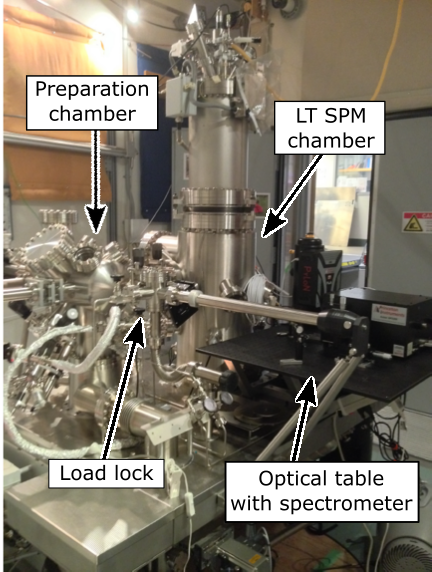
\includegraphics[width=0.55\textwidth]{pictures/microscope_labelled.png}
    \caption{Image of Omicron UHV LT SPM with optical access.}
    \label{fig:expsetup:omicron}
\end{figure}

The entire microscope is inside of an ultra-low vibration facility (dubbed ``the pod"), where it sits on a \SI{36}{tonne} concrete inertia block that is resting on six pneumatic isolators. To further decouple vibrations of the main building from the microscope, the pod is surrounded by a double-walled concrete enclosure containing acoustically isolating material, and rests on a foundation separate from the main building. Small feed-through openings allow wires to be passed from the microscope to a control unit outside the pod. The microscope can then be remotely operated using a computer in a separate control room. More details on the performance and design of the ultra-low vibration facility is given in reference \citep{macleod2015ultra}.

The microscope is composed of two main chambers: the preparation and the \acf{LT} chamber. The preparation chamber is typically at a base pressure of $\sim 1\times 10^{-10}$ mbar, minimizing contamination during sample preparation. In this chamber, the metallic substrates were cleaned by repeated sputtering and annealing. Decoupling layers of \ch{NaCl} were then deposited onto the surface using a home-built Knudsen evaporator. The substrates were then transferred into the \ac{LT} chamber for imaging and experimentation.

The \ac{LT} chamber is separated from the preparation chamber by a gate valve, and has a base pressure of $\sim 1\times 10^{-11}$ mbar. Samples are often stored in this chamber on a rotating carousel. The samples can be loaded into the \ac{SPM}, which is kept at $\sim \SI{4.3}{K}$ by a cryostat of \acf{LHe} surrounded by a \acf{LN2} bath. With the sample inside the \ac{SPM}, molecules were thermally deposited on the cold sample using an \ac{OMBE} evaporator. At such low temperatures, the molecules are more stable on insulating \ch{NaCl} layers, diffusing less, preventing aggregation and self-assembly. For more information on the equipment in the chambers, including the evaporators, and the sample design, refer to \citep{cochrane2017single, roussy2016coupling}. 

% A ceramic heater in the sample stage allows for mild annealing in the \ac{LT} chamber. 



\subsection{Scanning probe with optical access}

The imaging \ac{SPM} head is shown in \autoref{fig:expsetup:head}. The entire apparatus is suspended on damping springs, which can be clamped to the cryostat for sample transfer and faster cooling. The tip sits on a scanner, which is controlled by a coarse motor and piezoelectric motors. To begin an experiment, the tip was roughly approached to the sample using the coarse motor. An auto-approach function was then activated, taking a coarse step and extending the piezoelectric motor repeatedly until a tunnelling current was detected.

\begin{figure} [h]
    \centering
    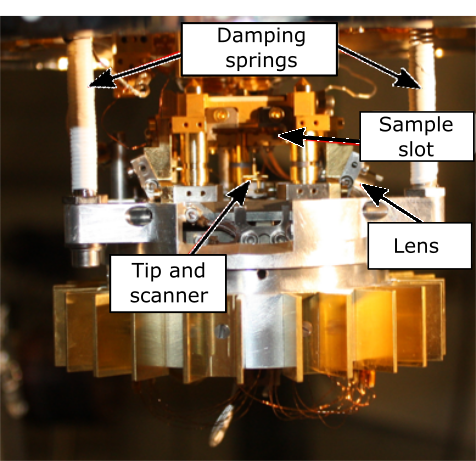
\includegraphics[width=0.45\textwidth]{pictures/spm_head_labelled.png}
    \caption{Image of the SPM head.}
    \label{fig:expsetup:head}
\end{figure}

There are two ports for optical access to the \ac{SPM} head. A camera used for coarse tip approach occupies one, while a home-built lens tube used for \ac{STML} occupies the other. A planoconvex sapphire lens (Melles-Griot) sits inside the lens tube, about \SI{18}{mm} from the tip-sample junction, at an angle of \SI{25}{\degree} from the sample. This geometry allows for collection of photons in about 5\% of the half solid angle above the sample. In order to maximize photon collection, the lens was focused at the tip-sample junction for the Ag(111) substrate, an \SI{8}{mm} tall top-hat crystal. The tip-sample junction is well approximated as a point source of light, and any shift from the lens focal point can weaken spectral features. When using the Au(111) thin film substrate, the height of the sample is different, resulting in weaker \ac{STML} signals.
% PXS-10.0-15.4-S

\begin{figure} [h]
    \centering
    \begin{subfigure}{.45\textwidth}
        \centering
        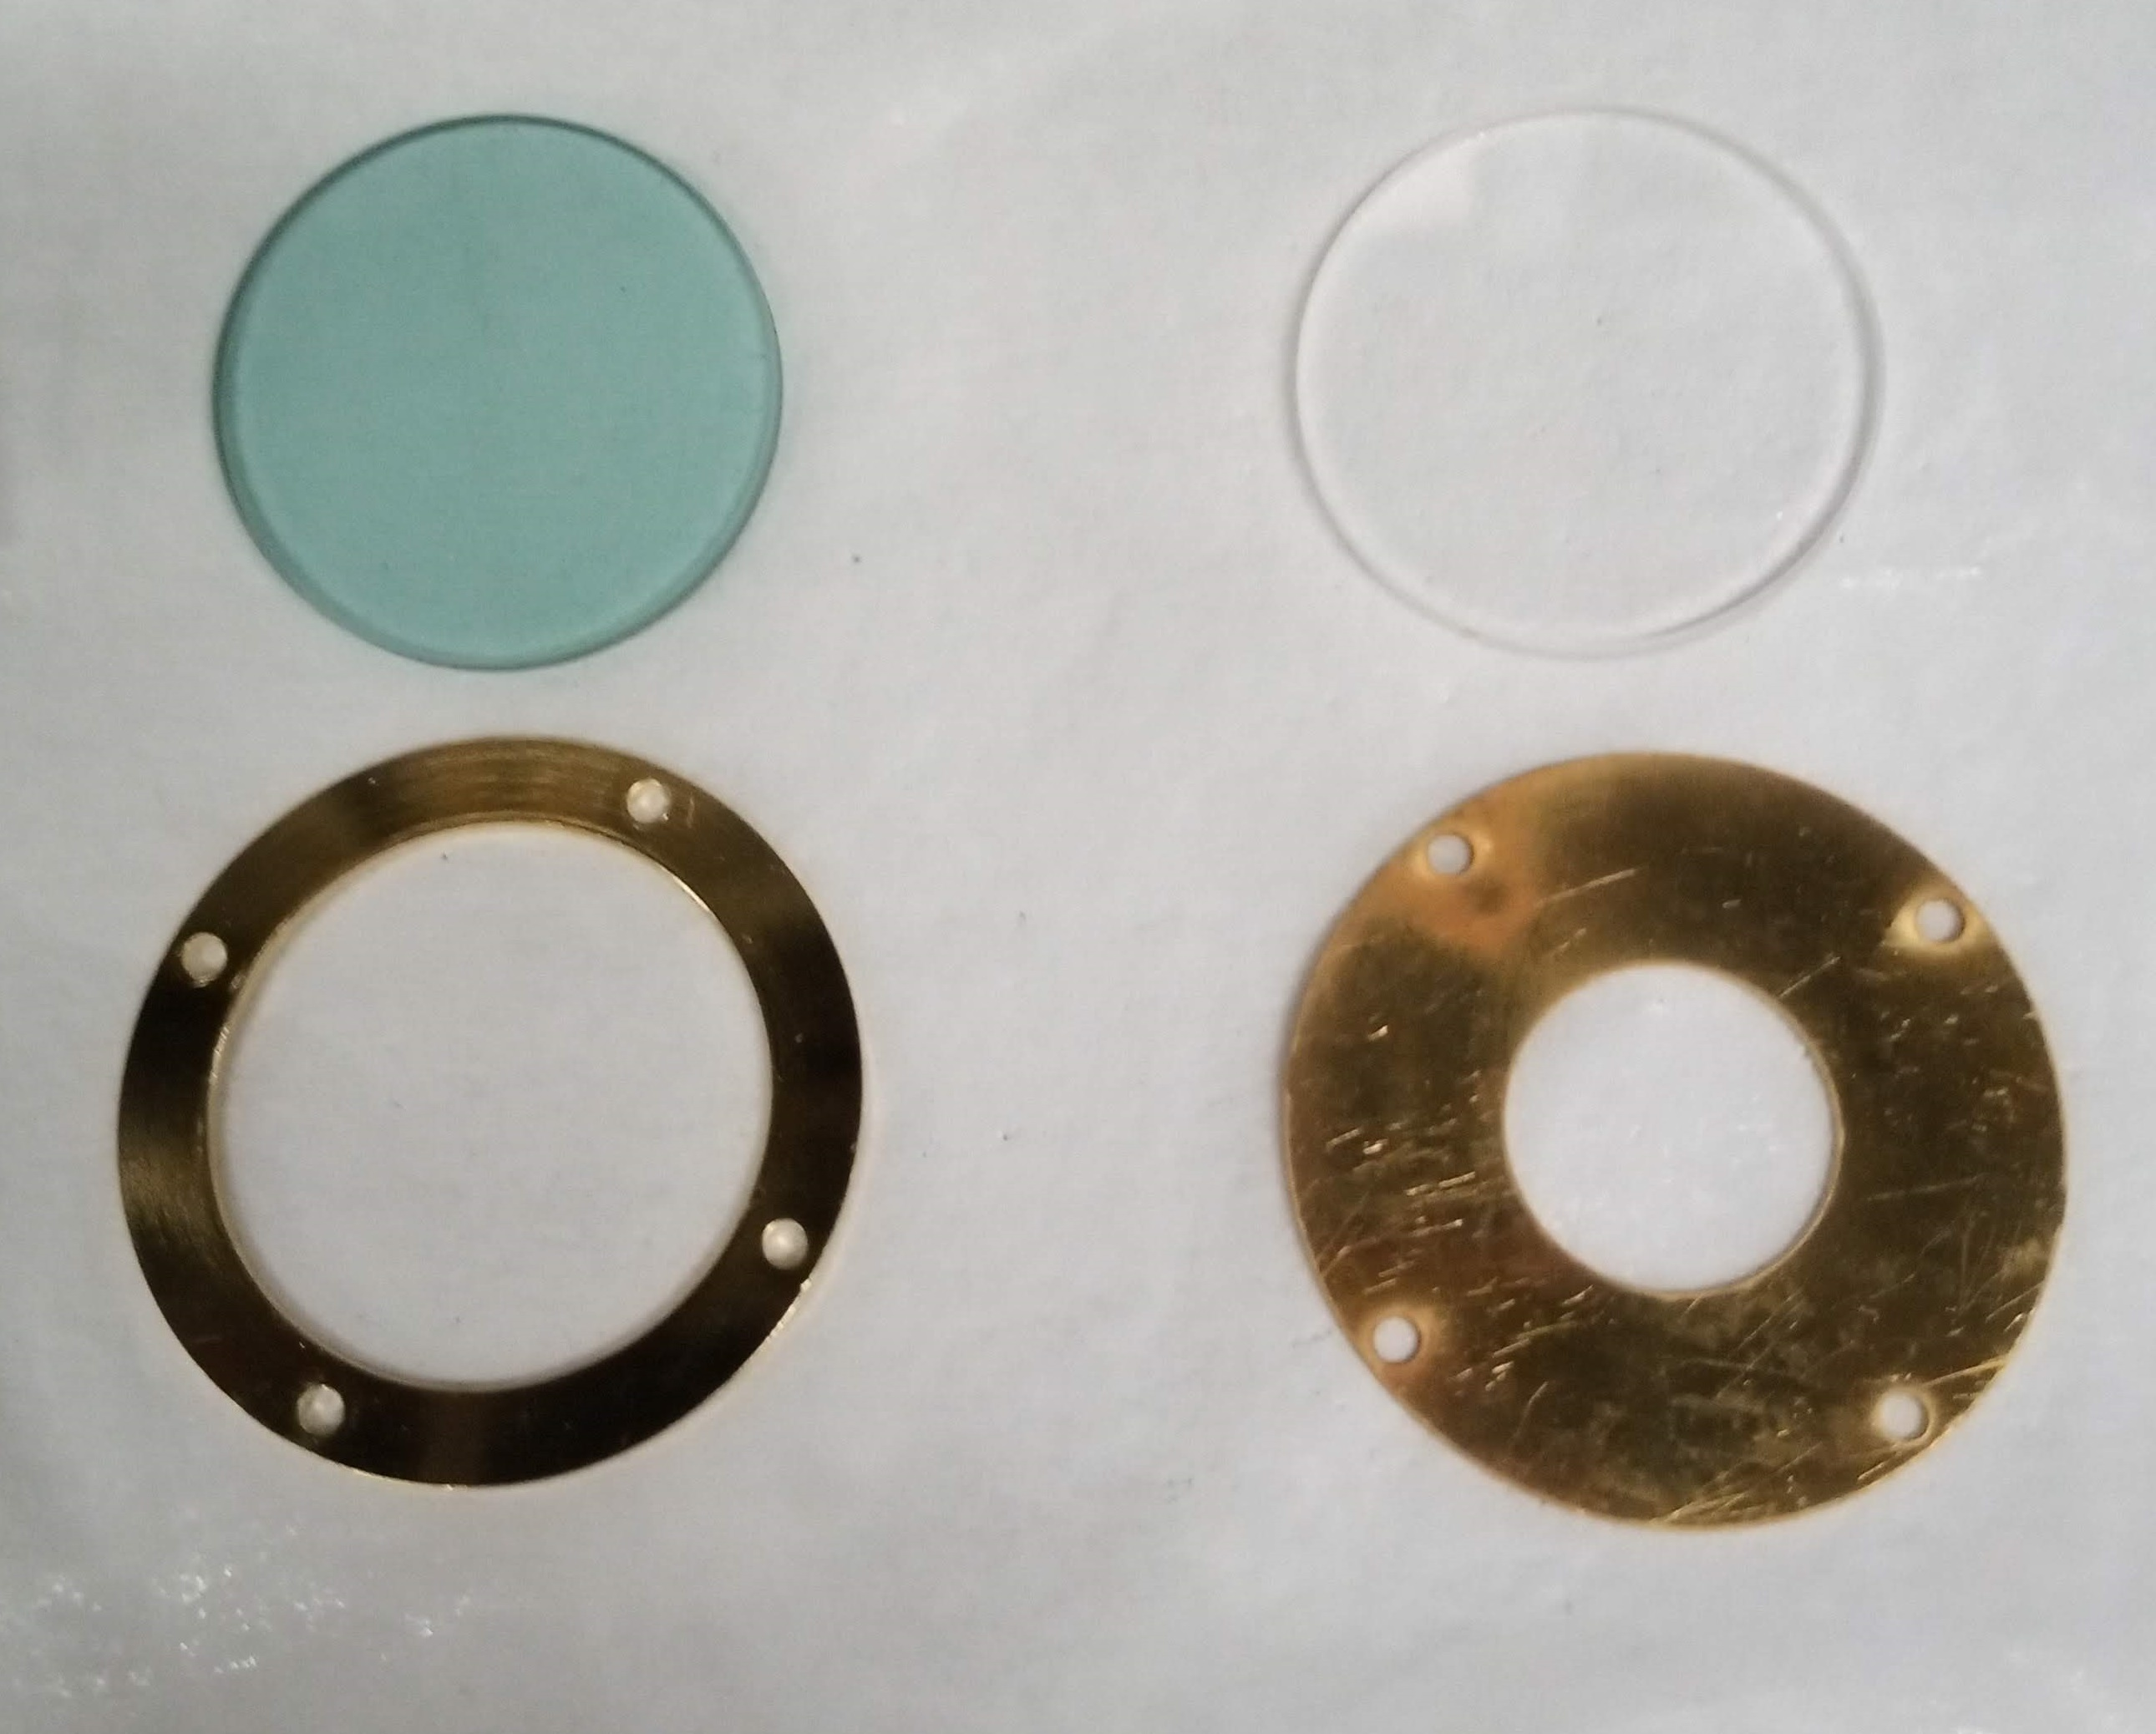
\includegraphics[width=\textwidth]{pictures/windows_filters_cropped.jpg}
        \captionsetup{width=\textwidth}
        \caption{\emph{Left:} KG5 IR filter with \SI{20}{mm} opening cover. \emph{Right:} WG41050 bandpass filter with \SI{12}{mm} opening cover. }
    \end{subfigure}
    
        \begin{subfigure}{.48\textwidth}
            \centering
            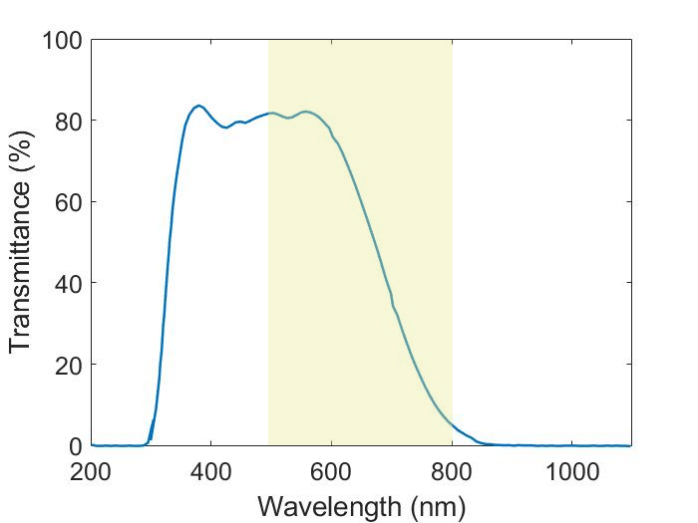
\includegraphics[width=\textwidth]{pictures/kg5_highlight.png}
            \caption{KG5 transmission curve.}
        \end{subfigure}
      \hfill
        \begin{subfigure}{.48\textwidth}
            \centering
            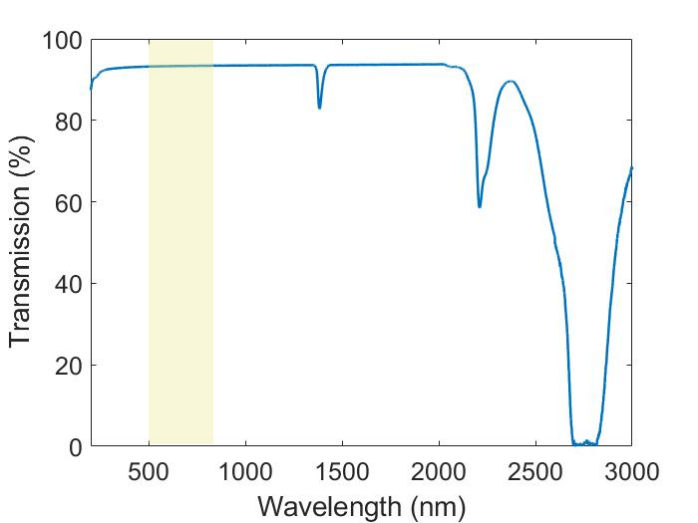
\includegraphics[width=\textwidth]{pictures/uvfs_highlight.png}
            \caption{WG41050 transmission curve.}
        \end{subfigure}
    
    \caption{Details of filters and windows. \textbf{(a)} IR and bandpass filters and respective windows. The transmission curves are shown in \textbf{(b)} and \textbf{(c)}, with region of interest, $\sim$\SI{500}{nm}--\SI{800}{nm}, highlighted.}
    \label{fig:expsetup:windows}
\end{figure}

The light from the lens then passes through ports in the two heat shields. These ports have KG5 \ac{IR} filters (SCHOTT) situated inside to reduce radiative heating of the \ac{SPM} head that would result in reduced cryostat hold time. Photon emission from organic semiconductors is often in the visible to near-\ac{IR} range, so the filters were later replaced with a WG41050 bandpass filter  (ThorLabs) that transmits wavelengths from at least \SI{300}{nm}--\SI{2}{\micro m}. The transmission curves of the filters are shown in \autoref{fig:expsetup:windows}. To counteract increased thermal energy entering the heat shields, the inner heat shield port opening was reduced from \SI{20}{mm} to \SI{12}{mm} in diameter using a \SI{0.4}{mm} thick gold-plated BeCu plate. After replacement of the filter, no noticeable changes were seen in the cryogenic hold time or base temperature. \emph{All \ac{STML} data was taken with the KG5 \ac{IR} filters in place}. Due to time constraints, \ac{STML} measurements were not repeated after the new window system was installed. The photons finally exit the \ac{LT} chamber through a Kodial vacuum viewport (VacGen), where they then enter an external optical setup mounted on the microscope. 



\subsection{Tip preparation}
\label{sec:expsetup:tip_prep}

In this thesis, a platinum/iridium (Pt/Ir) and a silver (Ag) tip were used. Below is a description of the tip preparation. The tips were then clamped into an Omicron tip holder and transferred into the microscope. 

The Pt/Ir tips were made by mechanically shearing a \SI{0.38}{mm} diameter wire. The Pt/Ir tip oxidizes relatively slowly and is stiff, meaning it can be conditioned by poking into the metal substrates, resulting in a Ag or Au terminated Pt/Ir tip. 

\begin{figure} [H]
    \centering
    % \begin{subfigure}{.2\textwidth}
    % 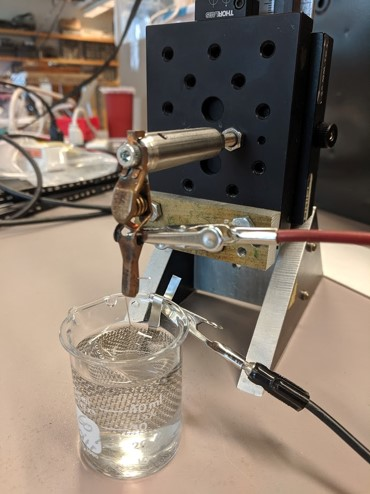
\includegraphics[width=\textwidth]{pictures/etch_setup.jpg}
    % \end{subfigure}
    % \hfill
    % \begin{subfigure}{.7\textwidth}
    % 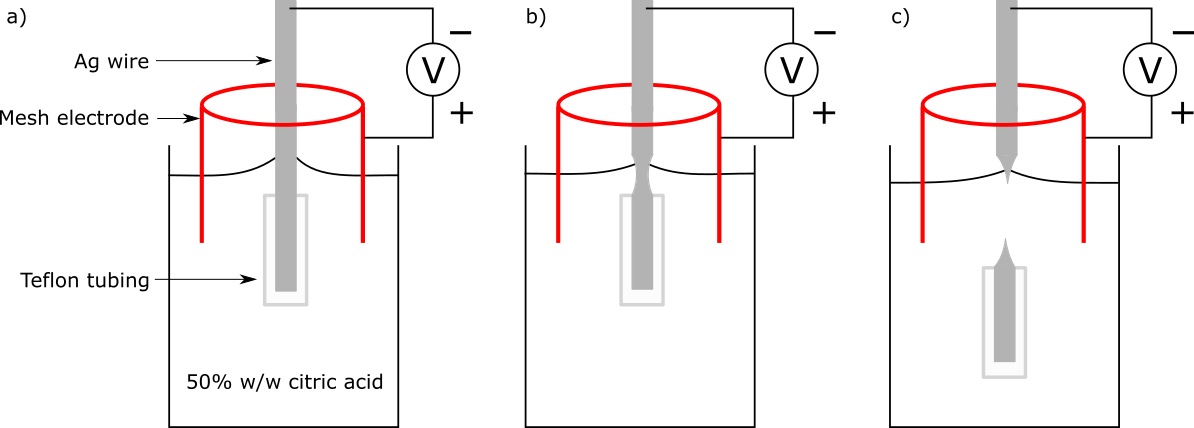
\includegraphics[width=\textwidth]{pictures/etch_diagram.png}
    % \end{subfigure}
    
    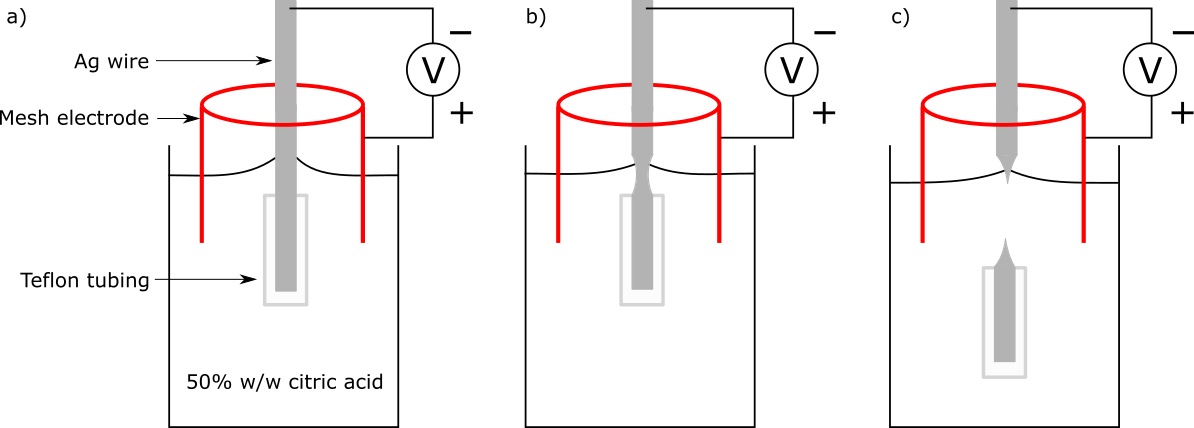
\includegraphics[width=0.9\textwidth]{pictures/etch_diagram.png}
    
    \caption{Diagram of Ag tip electrochemical etching setup. \textbf{(a)} Ag wire is suspended in acid with mesh electrode around it. An AC bias of \SI{39}{V} is applied with the negative terminal attached to the wire. Telfon tubing protects the bottom portion of the wire. \textbf{(b)} Preferential etching at the meniscus and shifting of the meniscus as etching progresses results in a tapered shape. \textbf{(c)} The dropped tip is used. Etching immediately stops for dropped tip once it is separated from the wire. }
    \label{fig:expsetup:etching}
\end{figure}

Ag is a material with low dielectric loss, making it optimal for \ac{STML}. Due to the importance of tip geometry in enhancing the luminescence signal, Ag tips were electrochemically etched, ensuring a well-defined and sharp tip shape. The procedures for Ag tip preparation are adapted from \citep{roussy2016coupling, zhang2011fabrication}. 

The etching setup is shown in \autoref{fig:expsetup:etching}. A \SI{0.404}{mm} diameter Ag wire was cleaned with acetone and isopropyl alcohol to give a clean etching surface. Teflon tubing covered the bottom $\sim$ \SI{3}{mm} of the wire to protect the region from chemical etching. The wire was then clamped and suspended in a solution of 50\% w/w citric acid in deionized water, with the meniscus about \SI{1.5}{mm} above the teflon protected region. A cylindrical mesh electrode was submerged into the solution with the wire in the centre to provide uniform etching on all sides. The wire was then etched using an \ac{AC} voltage source at \SI{39}{V}, with the negative terminal connected to the wire, and the ground terminal connected to the mesh electrode. 

\begin{figure} [h]
    \centering
    \begin{subfigure}[t]{0.35\textwidth}
    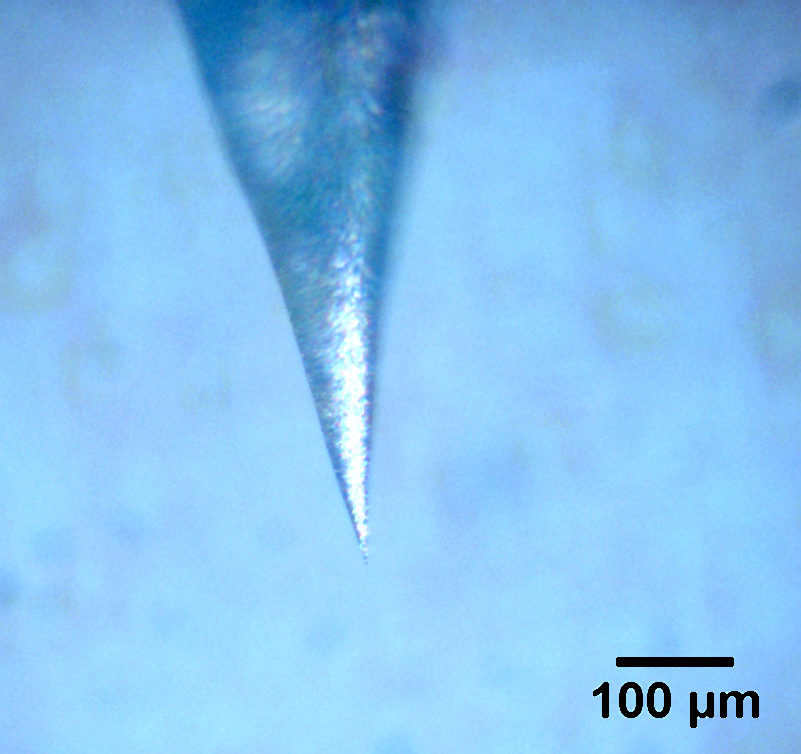
\includegraphics[width=\textwidth]{pictures/10x_meniscus_agtip_sb.png}
    \caption{}
    \end{subfigure}
    \hspace{0.5cm}
    \begin{subfigure}[t]{0.36\textwidth}
    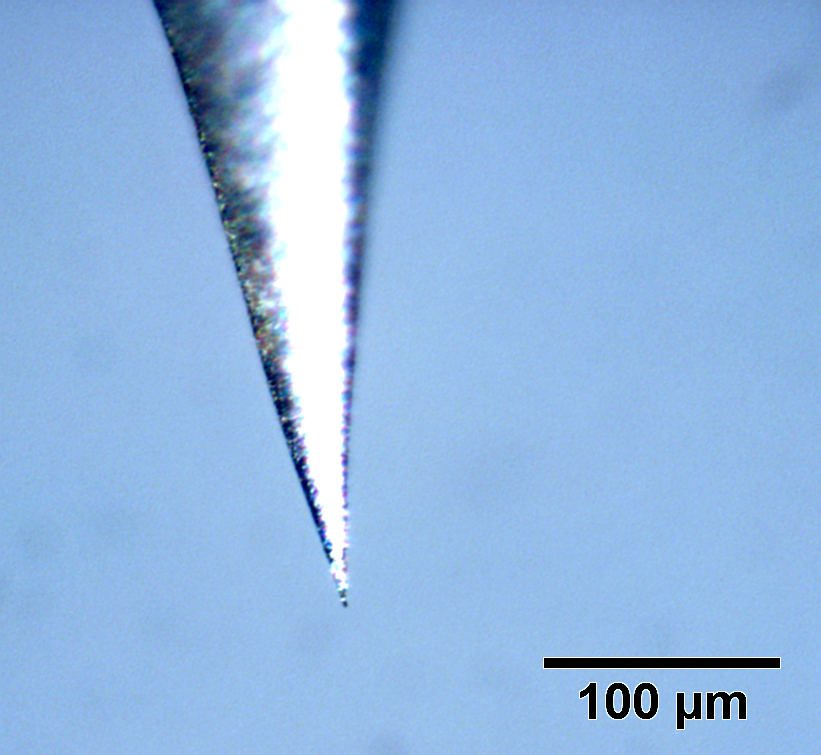
\includegraphics[width=\textwidth]{pictures/20x_meniscus_agtip_sb.png}
    \caption{}
    \end{subfigure}
    
    \caption{Ag tip imaged with optical microscope after etching. \textbf{(a)} is at 10x magnification, and \textbf{(b)} is at 20x magnification.}
    \label{fig:expsetup:image-plasmon}
\end{figure}

Etching typically took \SI{30}{min}. Surface tension effects and preferential etching at the meniscus produces a sharp metallic tip from the submerged portion of the wire, which drops into the solution, breaking electrical contact with the negative terminal and ending etching processes (\autoref{fig:expsetup:etching}). The tip was removed from the solution with the sharp side facing away from the meniscus, as the surface tension can bend the tip. The teflon tubing was removed, and the tip was rinsed in deionized water, followed by acetone and isopropyl alcohol. The tip was then examined with an optical microscope to ensure the tip was macroscopically sharp, and possessed a shiny metallic surface (\autoref{fig:expsetup:image-plasmon}). With the tip exposed to air, the Ag is susceptible to oxidation which can quench luminescence signals. If the tip passed inspection, it was immediately mounted and placed under vacuum in the microscope. We found the most success with Ag tips that were exposed to air for no longer than \SI{15}{min}.

\begin{figure}[H]
    \centering
    
    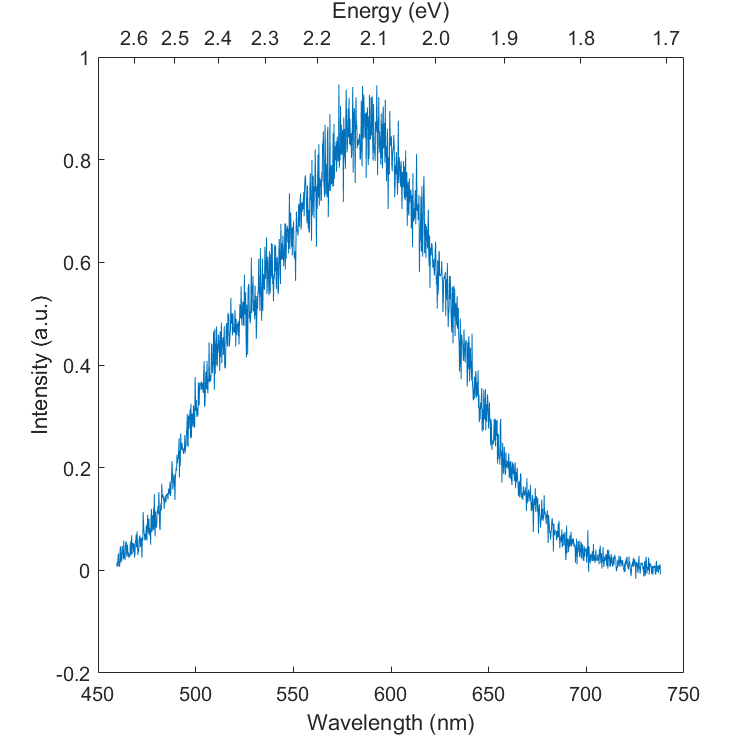
\includegraphics[width=0.6\textwidth]{pictures/ag111_plasmon.png}
    \caption[Plasmon emission with Ag tip on Ag(111) (\stmlparams{3}{200}{10}). Emission intensity $\sim 0.5$--$1.0$ a.u. is sufficient for STML experiments.]{Plasmon emission with Ag tip on Ag(111) (\stmlparams{3}{200}{10}). Emission intensity $\sim 0.5$--$1.0$ a.u. is sufficient for STML experiments.\footnotemark}
    
    \label{fig:expsetup:plasmon}
\end{figure}

\footnotetext{{Due to issues with intensity calibration on the spectrometer, the intensity of emission is given in arbitrary units rather than photon counts.}}

Due to the softness of Ag, it is extremely important that the tip does not crash into the surface. To prepare the tip for \ac{STML} experiments, the tip was repeatedly pulsed with voltages ranging from $5-\SI{10}{V}$ in order to remove residue and oxide from the tip. The shape of the tip was modified by piezo-controlled indentation into the metal substrate, ranging from 1$\SI{-10}{nm}$. With the optical setup aligned (discussed in the next section), the tip should demonstrate strong and broad plasmonic emission around $\sim \SI{600}{nm}$ on Ag(111) at bias voltage $V_b = \SI{3}{V}$, tunnelling current $I_t = \SI{200}{pA}$, and exposure time $t_x = \SI{10}{s}$ (\autoref{fig:expsetup:plasmon}). These parameters offer a baseline signal for later comparison.




\subsection{External optical setup}

Light collected by the lens inside the \ac{SPM} head exited the \ac{LT} chamber through a viewport. The external optical setup is shown in \autoref{fig:expsetup:optics}. A mirror mounted on the viewport directed the photons toward an optical table installed on the microscope. On the optical table, another mirror directed the light into a lens mounted on an \textit{xyz} micrometer stage, focusing the light into a spectrometer. The spectrometer energetically resolved the incoming photons, and the signal was detected with a \ac{LN2} cooled \ac{CCD}. The external optical setup was designed by T. Roussy \citep{roussy2016coupling}.

\begin{figure} [h]
    \centering
    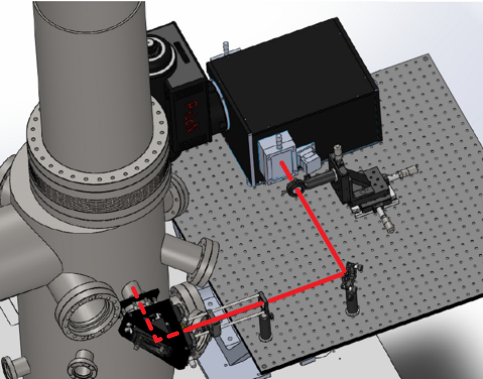
\includegraphics[width=0.8\textwidth]{pictures/optics_line.png}
    \caption{Diagram of external optics on optics table mounted on microscope. The red line represents the beam path.}
    \label{fig:expsetup:optics}
\end{figure}

Before starting any experiment, the \ac{CCD} was calibrated for each spectrometer grating using a mountable Hg lamp. The provided software uses the characteristic emission peaks of Hg to relate \ac{CCD} pixels to photon wavelength, with typical uncertainty values of $\pm$\SI{0.1}{nm}. Intensity calibration was not performed due to issues with the provided calibration lamp, hence the intensity of measured emissions are on an arbitrary scale rather than photon counts. However, comparison between relative peak intensities are still possible in the arbitrary scale.

In this work, two spectrometer gratings were used, with grating densities 300 gratings (gr)/mm and 600 gr/mm.\footnote{Some signal may be lost due to the imperfect reflectivity of the gratings. Reflectivity of the gratings at the regions of interest are around $70 - 80 \%$ \citep{princetongratings}} Higher grating density allows for higher resolution at the expense of spectral range. Once calibrated, all light sources in the room were covered or turned off and a background spectrum was taken. This background spectrum is subtracted from all experimental data, and accounts for thermal noise and stray light in the room.

The optical setup was then aligned to ensure that emission from the tip-sample junction entered the spectrometer. To begin, the lens on the optical table was removed, and the tip was coarse approached to the sample. The face of the spectrometer was illuminated such that a shadow of the slit could be seen on the surface of the metallic substrate. The shadow of the slit and the tip-sample junction were aligned, either by moving the tip or changing the angle of the two mirrors. With the tip-sample junction and spectrometer slit aligned, the lens can be mounted onto the micrometer stage. Shining light in through the camera port, the light reflected off the tip-sample junction can be focused into the spectrometer slit by adjusting the position of the lens.

During data acquisition, the tip was held at a point on the sample with a certain bias voltage ($V_b$) and tunnelling current ($I_t$). The spectrometer shutter was then opened for an exposure time ($t_x$). All measurements were done with the largest slit opening (\SI{3}{mm}) to maximize the amount of light entering the spectrometer. This comes at a cost: spectral features that are sharper than a \ac{FWHM} of \SI{3}{nm} (for the 300 gr/mm) or \SI{1}{nm} (for the 600 gr/mm) are broadened and not resolved \citep{princetonslit}. 



\section{Sample preparation}

Sample preparation involves cleaning the substrate, depositing the \ch{NaCl} film, and depositing the molecules. In this thesis, five different organic semiconducting molecules were studied, each with different deposition parameters. All sample preparation procedures will be discussed in detail.

\subsection*{Ag(111) substrate}

A top-hat silver crystal with (111) termination was the primary substrate used for experiments. The crystal surface was cleaned by sputtering for \SI{20}{\minute} using ionized \ch{Ar} gas, with ionizing potential $\sim \SI{1}{kV}$ and preparation chamber pressures at $P_{prep} \approx 3 \times 10^{-6}$ mbar. The substrate was then annealed using an e-beam heater at $T_{sub} = \SI{420}{\celsius}$ for another \SI{20}{\minute}. This was repeated 2--3 times depending on the status of the crystal surface.

A typical scan of a clean Ag(111) surface is seen in \autoref{fig:expsetup:Ag111}. When scanned with a sharp metallic tip, step heights are typically $\sim\SI{2}{\angstrom}$, and the \ac{STS} point spectra has a ``kink" at \SI{-67}{mV}. This corresponds to a step in the density of states, approximated by the normalized differential conductance, which is a result of the onset of the surface state of Ag(111) \citep{hovel2001modification}.

\begin{figure} [H]
    \centering
    \begin{subfigure}[t]{0.44\textwidth}
    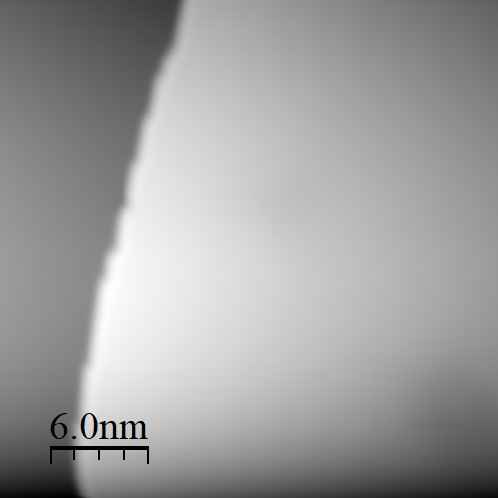
\includegraphics[width=\textwidth]{pictures/ag111_1V_10pA.jpg}
    \caption{}
    \end{subfigure}
    \hfill
    \begin{subfigure}[t]{0.53\textwidth}
        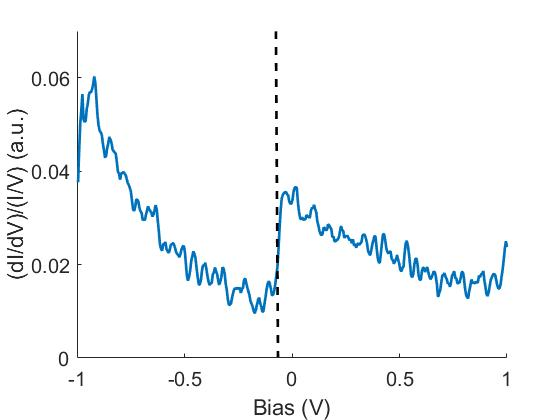
\includegraphics[width=\textwidth]{pictures/ag111_surface_state.jpg}
        \caption{}

    \end{subfigure}
    
    \caption{STM and STS of bare Ag(111) substrate. \textbf{(a)} STM topography (\stmparams{30}{30}{1}{10}). \textbf{(b)} Surface state of Ag(111), indicated at \SI{-67}{meV}, seen in normalized $dI/dV$.}
    
    \label{fig:expsetup:Ag111}
\end{figure}


\subsection*{Au(111) on Mica substrate}

As an alternate substrate, a thin film of (111) terminated gold on mica was used. The cleaning is similar to the procedures for Ag(111), but with sputtering potential $\sim \SI{0.75}{kV}$, and annealing temperature $T_{sub} = \SI{345}{\celsius}$.

An \ac{STM} image of the Au(111) thin film (\autoref{fig:expsetup:Au111}) shows a herringbone structure as a result of the reconstruction of the surface into regions of face centred cubic and hexagonal close packed atomic arrangements \citep{barth1990scanning}. Step heights on the surface are $\sim \SI{2}{\angstrom}$. The \ac{STS} spectra shows that the onset of the surface state is around $\SI{-450}{mV}$.

\begin{figure} [H]
    \centering
    \begin{subfigure}[t]{0.44\textwidth}
    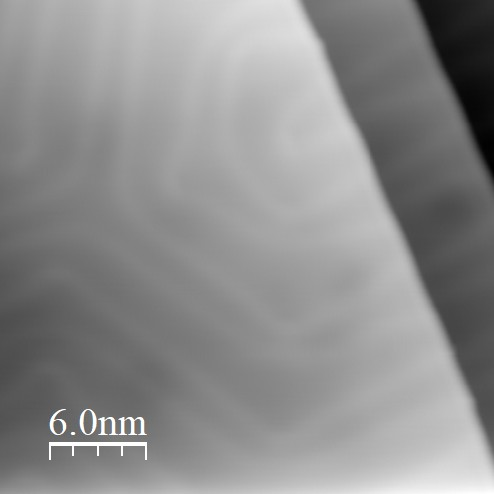
\includegraphics[width=\textwidth]{pictures/au111_1V_5pA.jpg}
    \caption{}
    \end{subfigure}
    \hfill
    \begin{subfigure}[t]{0.53\textwidth}
    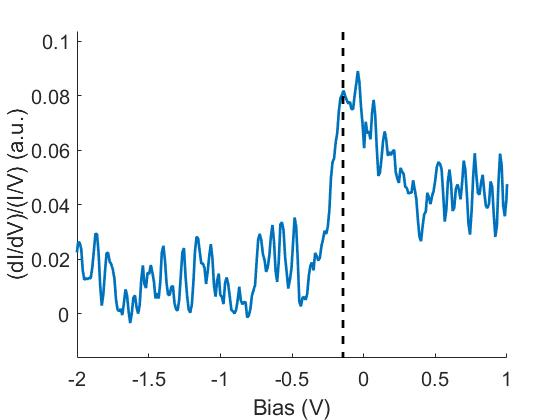
\includegraphics[width=\textwidth]{pictures/au111_surface_state.jpg}
    \caption{}
    \end{subfigure}
    
    \caption{STM and STS of bare Au(111) substrate. \textbf{(a)} STM topography (\stmparams{30}{30}{1}{5}). \textbf{(b)} Surface state of Au(111), indicated at \SI{-100}{meV}, seen in normalized $dI/dV$.}
    \label{fig:expsetup:Au111}
\end{figure}


\subsection*{NaCl deposition}

Films of \ch{NaCl}(001) were thermally deposited onto the metallic substrates. This insulating film partially decouples the molecule from the metallic substrate, while still allowing for tunnelling between the tip and sample \citep{repp2005molecules}. The decoupling is also necessary for \ac{STML} experiments, as emission from excitons in the molecule are quenched by electronic pathways between the molecule and the metal substrate.

\begin{figure} [H]
    \centering
    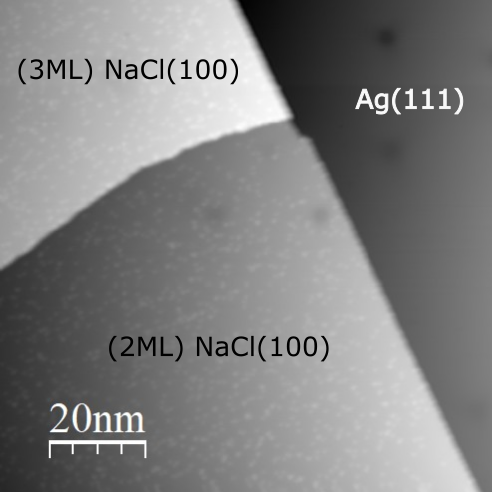
\includegraphics[width=0.5\textwidth]{pictures/nacl_example.png}
    \caption{STM image of 2 and 3ML NaCl on Ag(111) substrate (\stmparams{100}{100}{1}{10}). NaCl islands are identified by the step heights and surface state shifts. }
    \label{fig:expsetup:2-3NaCl}
\end{figure}

NaCl was thermally deposited using a home-built Knudsen cell. The thickness of the film can be controlled by deposition temperature, time, and substrate temperature. With the substrate held at $T_{sub} = \SI{100}{\celsius}$, NaCl was deposited for \SI{12}{\minute} with deposition temperature at approximately \SI{550}{\celsius}. 

\ac{STM} of bilayer and trilayer (2-\acf{ML} and 3\ac{ML}) NaCl on Ag(111) is shown in \autoref{fig:expsetup:2-3NaCl}, seen as rectangular terraces. The step height of 2\ac{ML} NaCl is around \SI{3}{\angstrom}, while 3\ac{ML} is at \SI{4.5}{\angstrom}. Experiments were carried out on the bilayer (2\ac{ML}) for better molecule and tip stability.

The presence of the NaCl layers energetically shifts the surface state of the metallic substrates (\autoref{fig:expsetup:NaClstate}). This signature in the \ac{STS} spectra is useful for determining whether a surface is metallic or insulating NaCl.

\begin{figure} [H]
    \centering
    \begin{subfigure}[t]{0.49\textwidth}
    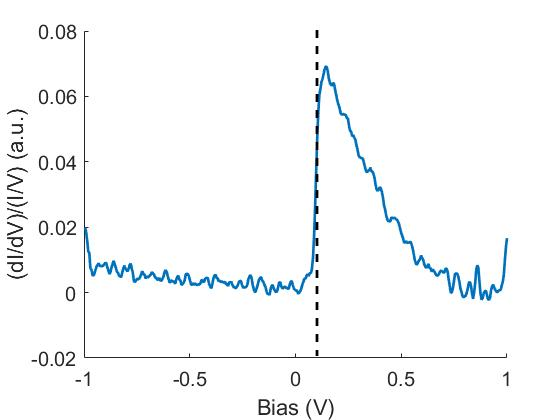
\includegraphics[width=\textwidth]{pictures/2mlnacl_ag111_surface_state.jpg}
    \caption{(2ML)NaCl/Ag(111)}
    \end{subfigure}
    \hfill
    \begin{subfigure}[t]{0.48\textwidth}
    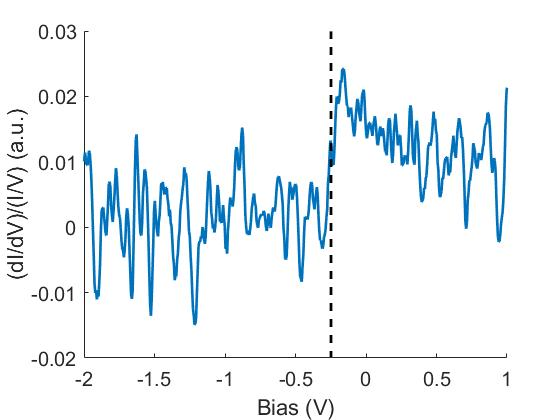
\includegraphics[width=\textwidth]{pictures/2mlnacl_au111_surface_state.jpg}
    \caption{(2ML)NaCl/Au(111)}
    \end{subfigure}
    
    \caption{Shifted surface state of substrates due to bilayer NaCl. \textbf{(a)} Surface state of Ag(111) shifted to \SI{+100}{meV}, and \textbf{(b)} Au(111) shifted to \SI{-250}{meV}.}
    \label{fig:expsetup:NaClstate}
\end{figure}

\subsection*{Molecule deposition}

Five different organic semiconducting molecules were used in our experiments (\autoref{fig:expsetup:molecules}). All molecules were deposited on a cold sample in the \ac{LT} chamber, with substrate temperature between \SI{4.3}{K} and \SI{4.5}{K}. The deposition parameters are summarized in \autoref{tab:expsetup:mol-dep}. 

\begin{figure} [H]
    \centering
    
\includegraphics[width=0.9\textwidth]{pictures/chemical_structures.png}
    \caption{Chemical structures of all molecules presented in this thesis. }
    \label{fig:expsetup:molecules}
\end{figure}

The \ac{HMAT} derivative molecules were synthesized by C. Tonge in the Hudson group in the chemistry department of \ac{UBC}. To obtain the deposition temperature for these molecules, thermogravimetric analysis was performed to give an approximate temperature at which the molecule begins to degrade. The molecules were then deposited onto the sample at approximately \SI{50}{\celsius} below the degradation temperature, and the sample scanned for presence of the molecules. The deposition temperature was ramped up in \SI{5}{\celsius} increments until the molecule was found on the surface.

\begin{table} [H]
\begin{center}
    \begin{tabular}{|c|c|c|} 
    \hline
        Molecule  &  \begin{tabular}[x]{@{}c@{}}Deposition\\temperature (\SI{}{\celsius})\end{tabular}   &  Time \\
        \hline
         PTCDA    &     325   & $\sim \SI{30}{s} $  \\
          ZnPc  &      370  & $\sim \SI{30}{s}$   \\
     \ch{F8ZnPc} &     370 & $\sim \SI{30}{s}$ \\
        HMAT-O   &    160  &    \SI{5}{\minute}\\
        HMAT-TZ  &    330   &  \SI{5}{\minute}\\
        HMAT-HZ  &    330  & \SI{10}{\minute}  \\
        \hline
    \end{tabular}
    \caption{Deposition temperature and time for each molecule used in experiments. Deposition times vary depending on the desired coverage. The times listed are for sparse coverages. The deposition may be repeated multiple times until coverage is sufficient. }
    \label{tab:expsetup:mol-dep}
    \end{center}
\end{table}


Unfortunately, the \ac{HMAT} derivatives were not stable at the sublimation temperature. Repeated degassing to remove impurities in the crucible resulted in continued deposition of molecular fragments. In order to preserve the integrity of the molecules, the deposition temperature was lowered, and the deposition time increased to the order of minutes. Final successful parameters are listed in \autoref{tab:expsetup:mol-dep}.













\section{Simulation methods}

\Acf{DFT} calculations were performed for the molecules, giving the molecular orbitals and energy levels of the isolated molecules. The results can be qualitatively compared to the experimental results. First, the chemical structures were drawn with the \textit{Avogadro} software \citep{hanwell2012avogadro}, which generated a file with the \ac{3D} coordinates of the atoms. As organic molecules can be flexible, different conformations were generated using the knowledge-based \ac{ETKDG} algorithm \citep{riniker2015better} built into the Python package \textit{RDKit} \citep{rdkit}. The \ac{ETKDG} algorithm generates molecular structures based on empirically defined libraries of torsional angles, ring conformations, and atomic distances. Molecular dynamics with the \ac{UFF} \citep{rappe1992uff} was used to calculate the energy of the conformations, and the lowest energy conformation was selected for \ac{DFT} calculations. Due to the many aromatic rings in the molecules we studied, the possible conformations were limited to planar structures, comparable to the planar configuration of the molecules on our metallic substrate.

Molecular orbitals and energy levels of free molecules were calculated using \ac{DFT} \emph{Gaussian 16} software package \citep{frisch2016gaussian}. The \ac{B3LYP} functional \citep{lee1988development, becke1993becke} and the 6-31G(d) \citep{frisch1984self} basis set were used for all calculations. A geometry optimization was performed on the conformer generated from molecular dynamics until the average force on all atoms were below $3\times 10^{-4}$ Ha/$r_{bohr}$. Finally, electronic structures of the fully relaxed molecules were calculated. The molecular orbitals were plotted with \textit{Avogadro}, with an electron density isosurface value of 0.02 electron/$r_{Bohr}^3$. The \ac{DOS} curves were extracted with the \textit{Multiwfn} software, with molecular states broadened by a Gaussian with a standard deviation of \SI{0.25}{eV}.

It is important to reiterate that the \ac{DFT} results can only be qualitatively compared with the experimental results. The \ac{DFT} calculations on the isolated molecules do not account for the interactions between the substrate and the molecule such as hybridization or van der Waals interactions. Additionally, geometrical changes to the molecule occur when they are adsorbed onto a surface, and a variety of stable conformations are possible.

%%%%%
